\documentclass[twoside]{book}

% Packages required by doxygen
\usepackage{fixltx2e}
\usepackage{calc}
\usepackage{doxygen}
\usepackage[export]{adjustbox} % also loads graphicx
\usepackage{graphicx}
\usepackage[utf8]{inputenc}
\usepackage{makeidx}
\usepackage{multicol}
\usepackage{multirow}
\PassOptionsToPackage{warn}{textcomp}
\usepackage{textcomp}
\usepackage[nointegrals]{wasysym}
\usepackage[table]{xcolor}

% NLS support packages
\usepackage[brazil]{babel}
% Font selection
\usepackage[T1]{fontenc}
\usepackage[scaled=.90]{helvet}
\usepackage{courier}
\usepackage{amssymb}
\usepackage{sectsty}
\renewcommand{\familydefault}{\sfdefault}
\allsectionsfont{%
  \fontseries{bc}\selectfont%
  \color{darkgray}%
}
\renewcommand{\DoxyLabelFont}{%
  \fontseries{bc}\selectfont%
  \color{darkgray}%
}
\newcommand{\+}{\discretionary{\mbox{\scriptsize$\hookleftarrow$}}{}{}}

% Page & text layout
\usepackage{geometry}
\geometry{%
  a4paper,%
  top=2.5cm,%
  bottom=2.5cm,%
  left=2.5cm,%
  right=2.5cm%
}
\tolerance=750
\hfuzz=15pt
\hbadness=750
\setlength{\emergencystretch}{15pt}
\setlength{\parindent}{0cm}
\setlength{\parskip}{3ex plus 2ex minus 2ex}
\makeatletter
\renewcommand{\paragraph}{%
  \@startsection{paragraph}{4}{0ex}{-1.0ex}{1.0ex}{%
    \normalfont\normalsize\bfseries\SS@parafont%
  }%
}
\renewcommand{\subparagraph}{%
  \@startsection{subparagraph}{5}{0ex}{-1.0ex}{1.0ex}{%
    \normalfont\normalsize\bfseries\SS@subparafont%
  }%
}
\makeatother

% Headers & footers
\usepackage{fancyhdr}
\pagestyle{fancyplain}
\fancyhead[LE]{\fancyplain{}{\bfseries\thepage}}
\fancyhead[CE]{\fancyplain{}{}}
\fancyhead[RE]{\fancyplain{}{\bfseries\leftmark}}
\fancyhead[LO]{\fancyplain{}{\bfseries\rightmark}}
\fancyhead[CO]{\fancyplain{}{}}
\fancyhead[RO]{\fancyplain{}{\bfseries\thepage}}
\fancyfoot[LE]{\fancyplain{}{}}
\fancyfoot[CE]{\fancyplain{}{}}
\fancyfoot[RE]{\fancyplain{}{\bfseries\scriptsize Gerado por Doxygen }}
\fancyfoot[LO]{\fancyplain{}{\bfseries\scriptsize Gerado por Doxygen }}
\fancyfoot[CO]{\fancyplain{}{}}
\fancyfoot[RO]{\fancyplain{}{}}
\renewcommand{\footrulewidth}{0.4pt}
\renewcommand{\chaptermark}[1]{%
  \markboth{#1}{}%
}
\renewcommand{\sectionmark}[1]{%
  \markright{\thesection\ #1}%
}

% Indices & bibliography
\usepackage{natbib}
\usepackage[titles]{tocloft}
\setcounter{tocdepth}{3}
\setcounter{secnumdepth}{5}
\makeindex

% Hyperlinks (required, but should be loaded last)
\usepackage{ifpdf}
\ifpdf
  \usepackage[pdftex,pagebackref=true]{hyperref}
\else
  \usepackage[ps2pdf,pagebackref=true]{hyperref}
\fi
\hypersetup{%
  colorlinks=true,%
  linkcolor=blue,%
  citecolor=blue,%
  unicode%
}

% Custom commands
\newcommand{\clearemptydoublepage}{%
  \newpage{\pagestyle{empty}\cleardoublepage}%
}

\usepackage{caption}
\captionsetup{labelsep=space,justification=centering,font={bf},singlelinecheck=off,skip=4pt,position=top}

%===== C O N T E N T S =====

\begin{document}

% Titlepage & ToC
\hypersetup{pageanchor=false,
             bookmarksnumbered=true,
             pdfencoding=unicode
            }
\pagenumbering{alph}
\begin{titlepage}
\vspace*{7cm}
\begin{center}%
{\Large Projeto P1 }\\
\vspace*{1cm}
{\large Gerado por Doxygen 1.8.14}\\
\end{center}
\end{titlepage}
\clearemptydoublepage
\pagenumbering{roman}
\tableofcontents
\clearemptydoublepage
\pagenumbering{arabic}
\hypersetup{pageanchor=true}

%--- Begin generated contents ---
\chapter{Projeto-\/1(P1)}
\label{md__c_1__users_lucas__idea_projects__projeto-1__r_e_a_d_m_e}
\Hypertarget{md__c_1__users_lucas__idea_projects__projeto-1__r_e_a_d_m_e}
C\+C3642 -\/ Orientação a Objetos

Nome\+: Lucas Pampolin Laheras RA\+: 22.\+117.\+055-\/8 
\chapter{Índice Hierárquico}
\section{Hierarquia de Classes}
Esta lista de hierarquias está parcialmente ordenada (ordem alfabética)\+:\begin{DoxyCompactList}
\item \contentsline{section}{Main}{\pageref{class_main}}{}
\item \contentsline{section}{Mundo}{\pageref{class_mundo}}{}
\item \contentsline{section}{Veiculo}{\pageref{class_veiculo}}{}
\begin{DoxyCompactList}
\item \contentsline{section}{Caminhao}{\pageref{class_caminhao}}{}
\item \contentsline{section}{Carro}{\pageref{class_carro}}{}
\item \contentsline{section}{Moto}{\pageref{class_moto}}{}
\end{DoxyCompactList}
\end{DoxyCompactList}

\chapter{Índice dos Componentes}
\section{Lista de Classes}
Aqui estão as classes, estruturas, uniões e interfaces e suas respectivas descrições\+:\begin{DoxyCompactList}
\item\contentsline{section}{\mbox{\hyperlink{class_caminhao}{Caminhao}} }{\pageref{class_caminhao}}{}
\item\contentsline{section}{\mbox{\hyperlink{class_carro}{Carro}} }{\pageref{class_carro}}{}
\item\contentsline{section}{\mbox{\hyperlink{class_main}{Main}} }{\pageref{class_main}}{}
\item\contentsline{section}{\mbox{\hyperlink{class_moto}{Moto}} }{\pageref{class_moto}}{}
\item\contentsline{section}{\mbox{\hyperlink{class_mundo}{Mundo}} }{\pageref{class_mundo}}{}
\item\contentsline{section}{\mbox{\hyperlink{class_veiculo}{Veiculo}} }{\pageref{class_veiculo}}{}
\end{DoxyCompactList}

\chapter{Classes}
\hypertarget{class_caminhao}{}\section{Referência da Classe Caminhao}
\label{class_caminhao}\index{Caminhao@{Caminhao}}
Diagrama de hierarquia para Caminhao\+:\begin{figure}[H]
\begin{center}
\leavevmode
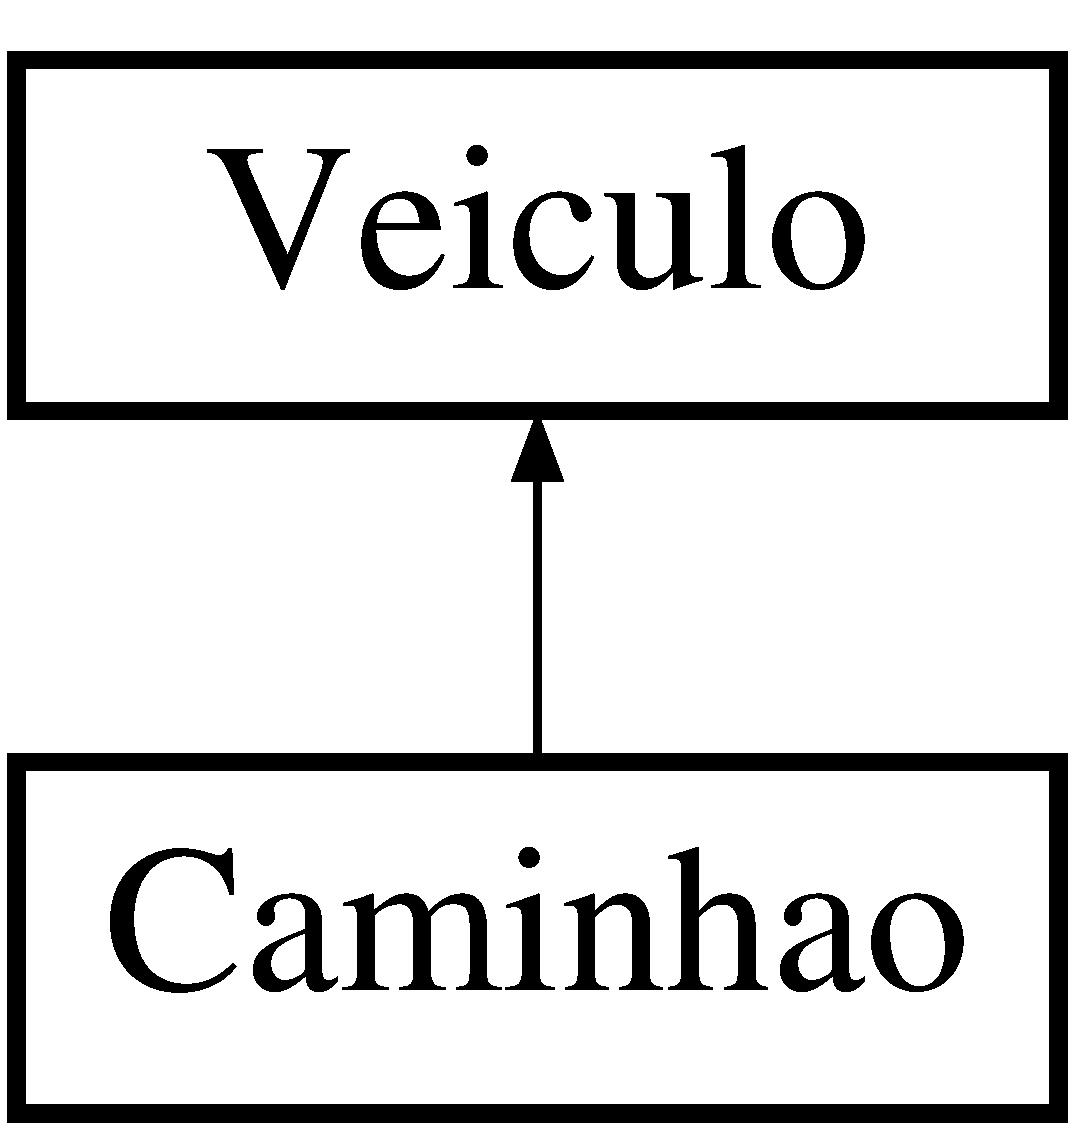
\includegraphics[height=2.000000cm]{class_caminhao}
\end{center}
\end{figure}
\subsection*{Métodos Públicos}
\begin{DoxyCompactItemize}
\item 
\mbox{\Hypertarget{class_caminhao_af533c39b3db0b14e7c404d4d91a88e47}\label{class_caminhao_af533c39b3db0b14e7c404d4d91a88e47}} 
\mbox{\hyperlink{class_caminhao_af533c39b3db0b14e7c404d4d91a88e47}{Caminhao}} ()
\begin{DoxyCompactList}\small\item\em Construtor de Caminhão com os valore de cor = 5 e velocidade = 1 fixos e a quantidade de toneladas variavel. \end{DoxyCompactList}\item 
\mbox{\Hypertarget{class_caminhao_a800cde90f61df345439b90e78552b026}\label{class_caminhao_a800cde90f61df345439b90e78552b026}} 
void \mbox{\hyperlink{class_caminhao_a800cde90f61df345439b90e78552b026}{set\+Toneladas}} (int \mbox{\hyperlink{class_caminhao_a76b6b066d32dac55e7b6e6669162b94e}{toneladas}})
\begin{DoxyCompactList}\small\item\em Método set para toneladas. \end{DoxyCompactList}\item 
\mbox{\Hypertarget{class_caminhao_a0d70fd366dda14b15b69fea764055001}\label{class_caminhao_a0d70fd366dda14b15b69fea764055001}} 
int \mbox{\hyperlink{class_caminhao_a0d70fd366dda14b15b69fea764055001}{get\+Toneladas}} ()
\begin{DoxyCompactList}\small\item\em Método get para toneladas. \end{DoxyCompactList}\end{DoxyCompactItemize}
\subsection*{Atributos Protegidos}
\begin{DoxyCompactItemize}
\item 
\mbox{\Hypertarget{class_caminhao_a76b6b066d32dac55e7b6e6669162b94e}\label{class_caminhao_a76b6b066d32dac55e7b6e6669162b94e}} 
int \mbox{\hyperlink{class_caminhao_a76b6b066d32dac55e7b6e6669162b94e}{toneladas}}
\begin{DoxyCompactList}\small\item\em Variavel que determina quantas toneladas o caminhão pode levar. \end{DoxyCompactList}\end{DoxyCompactItemize}
\subsection*{Outros membros herdados}


A documentação para essa classe foi gerada a partir do seguinte arquivo\+:\begin{DoxyCompactItemize}
\item 
C\+:/\+Users/lucas/\+Idea\+Projects/\+Projeto-\/1/Caminhao.\+java\end{DoxyCompactItemize}

\hypertarget{class_carro}{}\section{Referência da Classe Carro}
\label{class_carro}\index{Carro@{Carro}}
Diagrama de hierarquia para Carro\+:\begin{figure}[H]
\begin{center}
\leavevmode
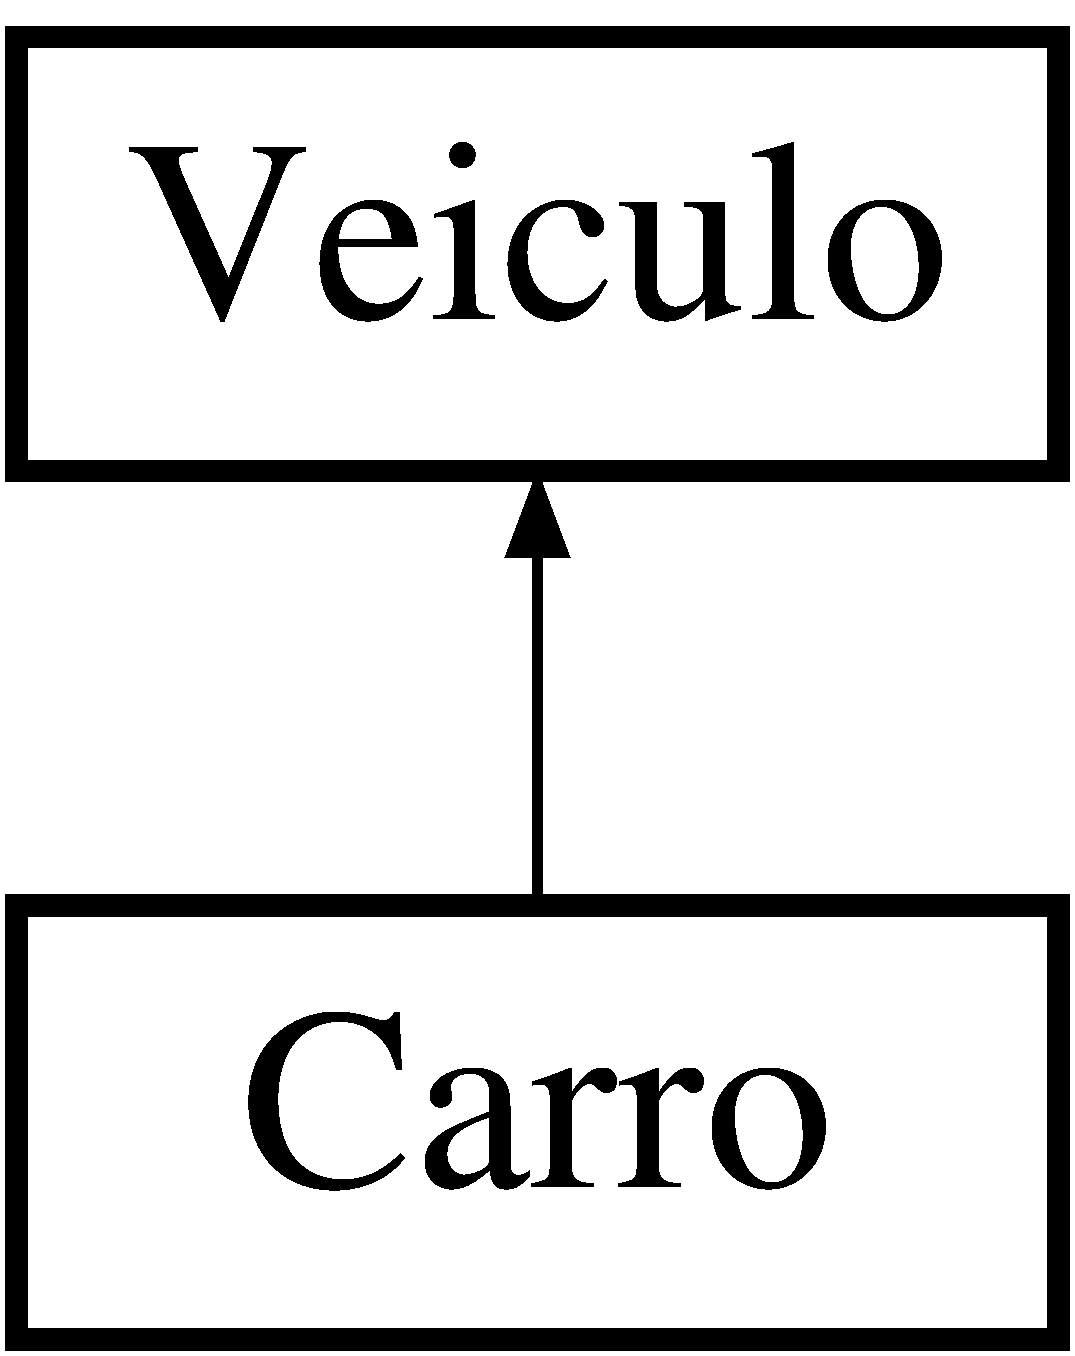
\includegraphics[height=2.000000cm]{class_carro}
\end{center}
\end{figure}
\subsection*{Métodos Públicos}
\begin{DoxyCompactItemize}
\item 
\mbox{\Hypertarget{class_carro_a853f79365b5c36491d34cf8f3815f75e}\label{class_carro_a853f79365b5c36491d34cf8f3815f75e}} 
\mbox{\hyperlink{class_carro_a853f79365b5c36491d34cf8f3815f75e}{Carro}} ()
\begin{DoxyCompactList}\small\item\em Construtor de \mbox{\hyperlink{class_carro}{Carro}} com os valore de cor = 4 e velocidade = 2 fixos e o tipo de carro que é varivel. \end{DoxyCompactList}\item 
\mbox{\Hypertarget{class_carro_aa2e79f3882d45b9558975402c204575f}\label{class_carro_aa2e79f3882d45b9558975402c204575f}} 
void \mbox{\hyperlink{class_carro_aa2e79f3882d45b9558975402c204575f}{set\+Tipo}} (int num)
\begin{DoxyCompactList}\small\item\em Seleciona qual tipo de carro é \end{DoxyCompactList}\item 
\mbox{\Hypertarget{class_carro_a44c3fde04be3cc309b9eac8b826c1560}\label{class_carro_a44c3fde04be3cc309b9eac8b826c1560}} 
String \mbox{\hyperlink{class_carro_a44c3fde04be3cc309b9eac8b826c1560}{get\+Tipo}} ()
\begin{DoxyCompactList}\small\item\em Retorna o tipo de carro. \end{DoxyCompactList}\end{DoxyCompactItemize}
\subsection*{Outros membros herdados}


A documentação para essa classe foi gerada a partir do seguinte arquivo\+:\begin{DoxyCompactItemize}
\item 
C\+:/\+Users/lucas/\+Idea\+Projects/\+Projeto-\/1/Carro.\+java\end{DoxyCompactItemize}

\hypertarget{class_main}{}\section{Referência da Classe Main}
\label{class_main}\index{Main@{Main}}
\subsection*{Membros Públicos Estáticos}
\begin{DoxyCompactItemize}
\item 
static void \mbox{\hyperlink{class_main_a8a5d0f827edddff706cc0e6740d0579a}{main}} (String\mbox{[}$\,$\mbox{]} args)
\end{DoxyCompactItemize}


\subsection{Métodos}
\mbox{\Hypertarget{class_main_a8a5d0f827edddff706cc0e6740d0579a}\label{class_main_a8a5d0f827edddff706cc0e6740d0579a}} 
\index{Main@{Main}!main@{main}}
\index{main@{main}!Main@{Main}}
\subsubsection{\texorpdfstring{main()}{main()}}
{\footnotesize\ttfamily static void Main.\+main (\begin{DoxyParamCaption}\item[{String \mbox{[}$\,$\mbox{]}}]{args }\end{DoxyParamCaption})\hspace{0.3cm}{\ttfamily [static]}}

Instancia o vetor array\+Moto

Instancia o vetor array\+Carro

Instancia o vetor array\+Caminhao

Instancia o m (mapa)

Adiciona ao vetor 10 veiculos de cada tipo e adiciona mais um ao contador de cada tipo de veiculo

Laco de repetição que irá rodar até não sobrar nenhum veiculo

A matriz mapa\+Atual recebe os valores padrões do mapa sem os veiculos

Move todos as motos

Move todos os carros

Move todos os caminhões

Insere no mapa todos as motos, carros e caminhões

Imprime a legenda com a quantidade de veículos

Imprime o mapa colorido

Pausa o programa durante 333 milisegundos

Move o cursor trita e oito linhas acima 

A documentação para essa classe foi gerada a partir do seguinte arquivo\+:\begin{DoxyCompactItemize}
\item 
C\+:/\+Users/lucas/\+Idea\+Projects/\+Projeto-\/1/Main.\+java\end{DoxyCompactItemize}

\hypertarget{class_moto}{}\section{Referência da Classe Moto}
\label{class_moto}\index{Moto@{Moto}}
Diagrama de hierarquia para Moto\+:\begin{figure}[H]
\begin{center}
\leavevmode
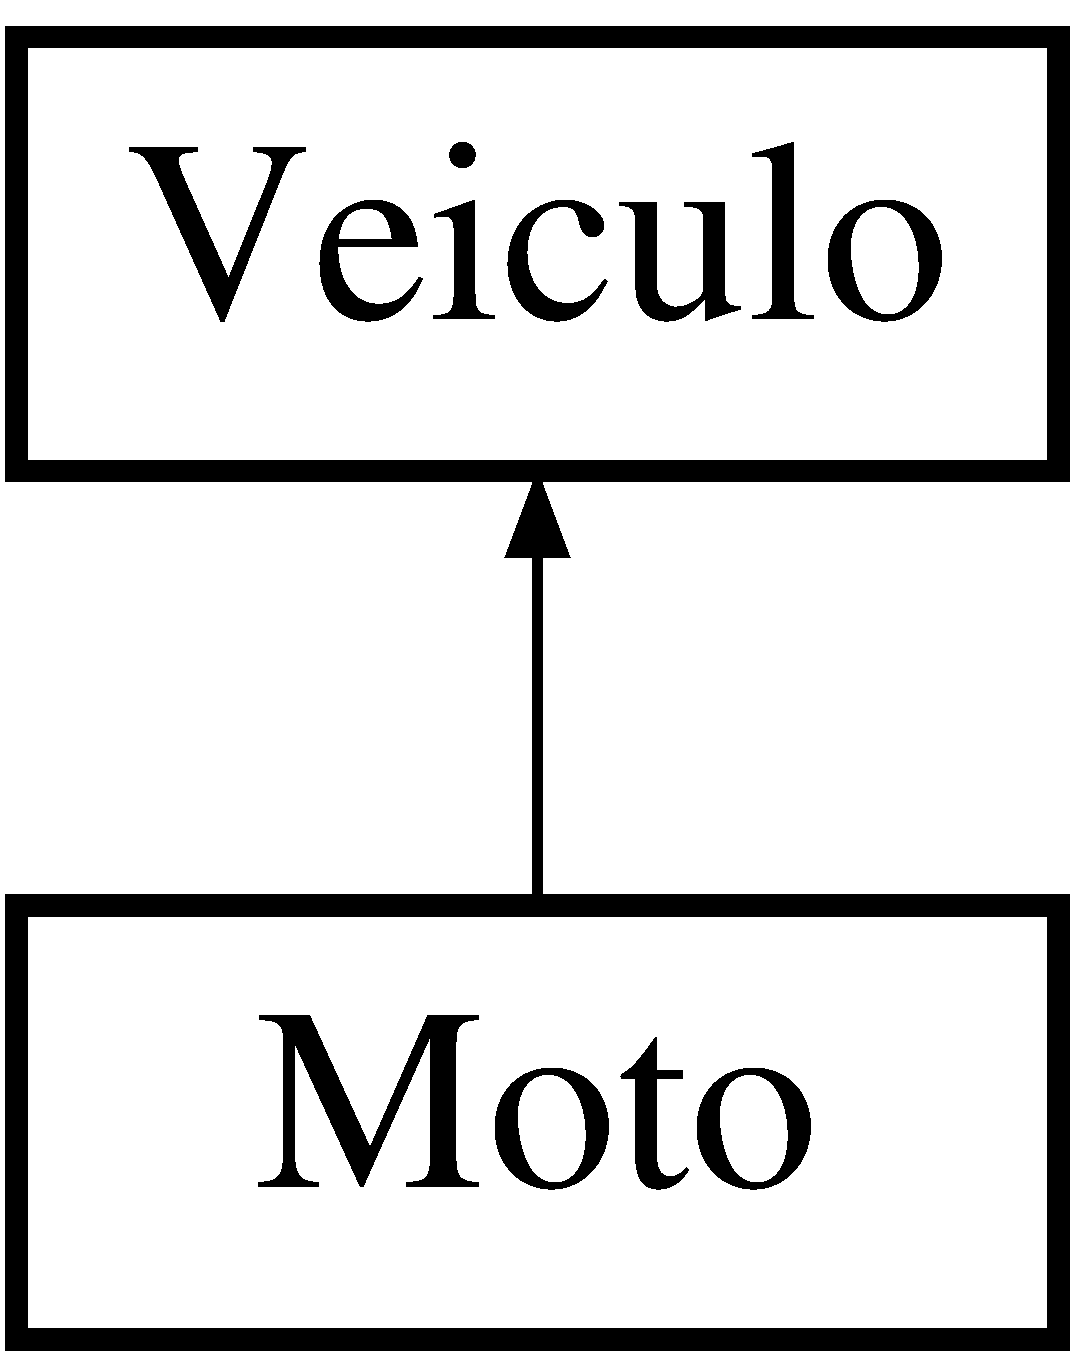
\includegraphics[height=2.000000cm]{class_moto}
\end{center}
\end{figure}
\subsection*{Métodos Públicos}
\begin{DoxyCompactItemize}
\item 
\mbox{\Hypertarget{class_moto_af900d6c1d6b9a69fb6b8bdb0c3401603}\label{class_moto_af900d6c1d6b9a69fb6b8bdb0c3401603}} 
\mbox{\hyperlink{class_moto_af900d6c1d6b9a69fb6b8bdb0c3401603}{Moto}} ()
\begin{DoxyCompactList}\small\item\em Construtor de Caminhão com os valore de cor = 3 e velocidade = 3 fixos e a quantidade de cilindradas que é variavel. \end{DoxyCompactList}\item 
\mbox{\Hypertarget{class_moto_ac379afd86f98c2def2e87b34abbe3f0c}\label{class_moto_ac379afd86f98c2def2e87b34abbe3f0c}} 
void \mbox{\hyperlink{class_moto_ac379afd86f98c2def2e87b34abbe3f0c}{set\+Cilindradas}} (int \mbox{\hyperlink{class_moto_ae62f5c23f1b1b77bbda2891971e0b169}{cilindradas}})
\begin{DoxyCompactList}\small\item\em Método set para cilindradas. \end{DoxyCompactList}\item 
\mbox{\Hypertarget{class_moto_aceb2f04f9b41595a26c57963bc115c61}\label{class_moto_aceb2f04f9b41595a26c57963bc115c61}} 
int \mbox{\hyperlink{class_moto_aceb2f04f9b41595a26c57963bc115c61}{get\+Cilindradas}} ()
\begin{DoxyCompactList}\small\item\em Método get para cilindradas. \end{DoxyCompactList}\end{DoxyCompactItemize}
\subsection*{Atributos Públicos}
\begin{DoxyCompactItemize}
\item 
\mbox{\Hypertarget{class_moto_ae62f5c23f1b1b77bbda2891971e0b169}\label{class_moto_ae62f5c23f1b1b77bbda2891971e0b169}} 
int \mbox{\hyperlink{class_moto_ae62f5c23f1b1b77bbda2891971e0b169}{cilindradas}}
\begin{DoxyCompactList}\small\item\em Variavel que determina quantas cilindradas a moto pode ter. \end{DoxyCompactList}\end{DoxyCompactItemize}
\subsection*{Outros membros herdados}


A documentação para essa classe foi gerada a partir do seguinte arquivo\+:\begin{DoxyCompactItemize}
\item 
C\+:/\+Users/lucas/\+Idea\+Projects/\+Projeto-\/1/Moto.\+java\end{DoxyCompactItemize}

\hypertarget{class_mundo}{}\section{Referência da Classe Mundo}
\label{class_mundo}\index{Mundo@{Mundo}}
\subsection*{Métodos Públicos}
\begin{DoxyCompactItemize}
\item 
\mbox{\Hypertarget{class_mundo_ae3801a0a633ad3475456c67639561105}\label{class_mundo_ae3801a0a633ad3475456c67639561105}} 
\mbox{\hyperlink{class_mundo_ae3801a0a633ad3475456c67639561105}{Mundo}} ()
\begin{DoxyCompactList}\small\item\em Construtor do mundo que inicia o mapa como padrão. \end{DoxyCompactList}\item 
void \mbox{\hyperlink{class_mundo_a1df37efee05155963d963b7f3ca07508}{imprime\+Mapa}} ()
\begin{DoxyCompactList}\small\item\em Método que imprime o mapa colorido. \end{DoxyCompactList}\item 
void \mbox{\hyperlink{class_mundo_ae896c013603704a78e4e9ca0c3b96356}{verifica\+Colisao\+E\+Insere\+No\+Mapa}} (Array\+List$<$ \mbox{\hyperlink{class_moto}{Moto}} $>$ array\+Moto, Array\+List$<$ \mbox{\hyperlink{class_carro}{Carro}} $>$ array\+Carro, Array\+List$<$ \mbox{\hyperlink{class_caminhao}{Caminhao}} $>$ array\+Caminhao)
\begin{DoxyCompactList}\small\item\em Verifica se há colisão entre veiculos e insere os veiculos no mapa (matriz) \end{DoxyCompactList}\item 
\mbox{\Hypertarget{class_mundo_a1be59b32572a7a8a40fa84737722e015}\label{class_mundo_a1be59b32572a7a8a40fa84737722e015}} 
void \mbox{\hyperlink{class_mundo_a1be59b32572a7a8a40fa84737722e015}{reinicia\+Mapa}} ()
\begin{DoxyCompactList}\small\item\em Iguala o mapa\+Atual à matriz padrão de 37 x 37, sendo 0 = nada, limite = 1, fabrica = 2, moto = 3, carro = 4, caminhão = 5. \end{DoxyCompactList}\item 
\mbox{\Hypertarget{class_mundo_acc3a26a242cfe494033e8f36bad5648b}\label{class_mundo_acc3a26a242cfe494033e8f36bad5648b}} 
int \mbox{\hyperlink{class_mundo_acc3a26a242cfe494033e8f36bad5648b}{get\+Adciona\+Caminhao}} ()
\begin{DoxyCompactList}\small\item\em Retorna o valor total de caminhões adicionados. \end{DoxyCompactList}\item 
\mbox{\Hypertarget{class_mundo_ac4e9fdfe30a81bf82f1eedf4b990c96a}\label{class_mundo_ac4e9fdfe30a81bf82f1eedf4b990c96a}} 
int \mbox{\hyperlink{class_mundo_ac4e9fdfe30a81bf82f1eedf4b990c96a}{get\+Adciona\+Carro}} ()
\begin{DoxyCompactList}\small\item\em Retorna o valor total de carros adicionados. \end{DoxyCompactList}\item 
\mbox{\Hypertarget{class_mundo_a7fb9d6c8df95d88eae88ed3d15f0195e}\label{class_mundo_a7fb9d6c8df95d88eae88ed3d15f0195e}} 
int \mbox{\hyperlink{class_mundo_a7fb9d6c8df95d88eae88ed3d15f0195e}{get\+Adciona\+Moto}} ()
\begin{DoxyCompactList}\small\item\em Retorna o valor total de motos adicionados. \end{DoxyCompactList}\item 
\mbox{\Hypertarget{class_mundo_ad2eb05e9209d3c30bf0514f0a24a502a}\label{class_mundo_ad2eb05e9209d3c30bf0514f0a24a502a}} 
int \mbox{\hyperlink{class_mundo_ad2eb05e9209d3c30bf0514f0a24a502a}{get\+Deleta\+Caminhao}} ()
\begin{DoxyCompactList}\small\item\em Retorna o valor total de caminhões deletados. \end{DoxyCompactList}\item 
\mbox{\Hypertarget{class_mundo_a999bc3ec64b4daed18ab28ad6657c56c}\label{class_mundo_a999bc3ec64b4daed18ab28ad6657c56c}} 
int \mbox{\hyperlink{class_mundo_a999bc3ec64b4daed18ab28ad6657c56c}{get\+Deleta\+Carro}} ()
\begin{DoxyCompactList}\small\item\em Retorna o valor total de carros deletados. \end{DoxyCompactList}\item 
\mbox{\Hypertarget{class_mundo_a80d1b5b8e454f2d218c3dbfb6e344d1a}\label{class_mundo_a80d1b5b8e454f2d218c3dbfb6e344d1a}} 
int \mbox{\hyperlink{class_mundo_a80d1b5b8e454f2d218c3dbfb6e344d1a}{get\+Deleta\+Moto}} ()
\begin{DoxyCompactList}\small\item\em Retorna o valor total de motos deletados. \end{DoxyCompactList}\item 
\mbox{\Hypertarget{class_mundo_a99e8d3c4c8eb354b5df7a8d3ea6a5f26}\label{class_mundo_a99e8d3c4c8eb354b5df7a8d3ea6a5f26}} 
void \mbox{\hyperlink{class_mundo_a99e8d3c4c8eb354b5df7a8d3ea6a5f26}{adciona\+Caminhao}} ()
\begin{DoxyCompactList}\small\item\em Adiciona um caminhão pro contador. \end{DoxyCompactList}\item 
\mbox{\Hypertarget{class_mundo_a9db53933148e177aa218415969de95fc}\label{class_mundo_a9db53933148e177aa218415969de95fc}} 
void \mbox{\hyperlink{class_mundo_a9db53933148e177aa218415969de95fc}{adciona\+Carro}} ()
\begin{DoxyCompactList}\small\item\em Adiciona um carro pro contador. \end{DoxyCompactList}\item 
\mbox{\Hypertarget{class_mundo_a4176d036c7c8c337938c8e41f4048a32}\label{class_mundo_a4176d036c7c8c337938c8e41f4048a32}} 
void \mbox{\hyperlink{class_mundo_a4176d036c7c8c337938c8e41f4048a32}{adciona\+Moto}} ()
\begin{DoxyCompactList}\small\item\em Adiciona uma moto pro contador. \end{DoxyCompactList}\end{DoxyCompactItemize}


\subsection{Métodos}
\mbox{\Hypertarget{class_mundo_a1df37efee05155963d963b7f3ca07508}\label{class_mundo_a1df37efee05155963d963b7f3ca07508}} 
\index{Mundo@{Mundo}!imprime\+Mapa@{imprime\+Mapa}}
\index{imprime\+Mapa@{imprime\+Mapa}!Mundo@{Mundo}}
\subsubsection{\texorpdfstring{imprime\+Mapa()}{imprimeMapa()}}
{\footnotesize\ttfamily void Mundo.\+imprime\+Mapa (\begin{DoxyParamCaption}{ }\end{DoxyParamCaption})}



Método que imprime o mapa colorido. 

Pinta de preto

Pinta de cinza claro

Pinta de magenta

Pinta de vermelho

Pinta de verde

Pinta de azul \mbox{\Hypertarget{class_mundo_ae896c013603704a78e4e9ca0c3b96356}\label{class_mundo_ae896c013603704a78e4e9ca0c3b96356}} 
\index{Mundo@{Mundo}!verifica\+Colisao\+E\+Insere\+No\+Mapa@{verifica\+Colisao\+E\+Insere\+No\+Mapa}}
\index{verifica\+Colisao\+E\+Insere\+No\+Mapa@{verifica\+Colisao\+E\+Insere\+No\+Mapa}!Mundo@{Mundo}}
\subsubsection{\texorpdfstring{verifica\+Colisao\+E\+Insere\+No\+Mapa()}{verificaColisaoEInsereNoMapa()}}
{\footnotesize\ttfamily void Mundo.\+verifica\+Colisao\+E\+Insere\+No\+Mapa (\begin{DoxyParamCaption}\item[{Array\+List$<$ \mbox{\hyperlink{class_moto}{Moto}} $>$}]{array\+Moto,  }\item[{Array\+List$<$ \mbox{\hyperlink{class_carro}{Carro}} $>$}]{array\+Carro,  }\item[{Array\+List$<$ \mbox{\hyperlink{class_caminhao}{Caminhao}} $>$}]{array\+Caminhao }\end{DoxyParamCaption})}



Verifica se há colisão entre veiculos e insere os veiculos no mapa (matriz) 

Laço que percorre todo vetor da moto

O x recebe o valor da posição horizontal do veículo

O y recebe o valor da vertical posição do veículo

Se no local da moto estiver vazio ou for uma borda, coloca a moto na matriz

Se no local da moto é uma fábrica, coloca na matriz e verifica se já estava na fábrica e se ela não estivesse duplica e adiciona no contador de adicionados

Se no local da moto tem outra moto, encontra a moto que está nessa posição, destrói as duas e adiciona no contador de deletados

O x recebe o valor da posição horizontal do veículo

O y recebe o valor da vertical posição do veículo

Se no local do carro estiver vazio ou for uma borda, coloca ele na matriz

Se no local do carro é uma fábrica, coloca na matriz e verifica se já estava na fábrica e se ele não estivesse duplica e adiciona no contador de adicionados

Se no local do carro tem uma moto, encontra a moto que está nessa posição, destrói e adiciona no contador de deletados

Se no local do carro tem outro carro, encontra o carro que está nessa posição, destrói os dois e adiciona no contador de deletados

Laço que percorre todo vetor do cominhao

O x recebe o valor da posição horizontal do veículo

O y recebe o valor da vertical posição do veículo

Se no local do caminhão estiver vazio ou for uma borda, coloca ele na matriz

Se no local do caminhão é uma fábrica, coloca na matriz e verifica se já estava na fábrica e se ele não estivesse duplica e adiciona no contador de adicionados

Se no local do caminhão tem uma moto, encontra a moto que está nessa posição, destrói e adiciona no contador de deletados

Se no local do caminhão tem um carro, encontra o carro que está nessa posição, destrói e adiciona no contador de deletados

Se no local do carro tem outro caminhão, encontra o caminhão que está nessa posição, destrói os dois e adiciona no contador de deletados 

A documentação para essa classe foi gerada a partir do seguinte arquivo\+:\begin{DoxyCompactItemize}
\item 
C\+:/\+Users/lucas/\+Idea\+Projects/\+Projeto-\/1/Mundo.\+java\end{DoxyCompactItemize}

\hypertarget{class_veiculo}{}\section{Referência da Classe Veiculo}
\label{class_veiculo}\index{Veiculo@{Veiculo}}
Diagrama de hierarquia para Veiculo\+:\begin{figure}[H]
\begin{center}
\leavevmode
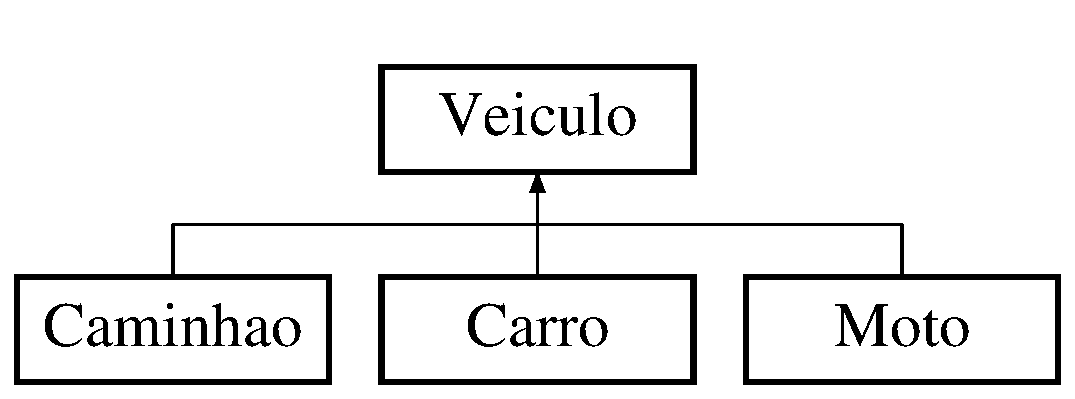
\includegraphics[height=2.000000cm]{class_veiculo}
\end{center}
\end{figure}
\subsection*{Métodos Públicos}
\begin{DoxyCompactItemize}
\item 
\mbox{\Hypertarget{class_veiculo_a5ea5d42f464f3f8844a793c4e144c2c2}\label{class_veiculo_a5ea5d42f464f3f8844a793c4e144c2c2}} 
\mbox{\hyperlink{class_veiculo_a5ea5d42f464f3f8844a793c4e144c2c2}{Veiculo}} (int \mbox{\hyperlink{class_veiculo_aad500265aeb92689ca66ec5bd87787a9}{cor}}, int \mbox{\hyperlink{class_veiculo_a2edf5e3132b1c2504c441dc095dc7e0e}{velocidade}})
\begin{DoxyCompactList}\small\item\em Construtor de veículo. \end{DoxyCompactList}\item 
void \mbox{\hyperlink{class_veiculo_ab7fc7e6551ab238df0fb51a1a5c7d66f}{set\+Cor}} (int \mbox{\hyperlink{class_veiculo_aad500265aeb92689ca66ec5bd87787a9}{cor}})
\begin{DoxyCompactList}\small\item\em Métodos set. \end{DoxyCompactList}\item 
void \mbox{\hyperlink{class_veiculo_a45be3eedbb5c60b9f422f7a7f9f145cd}{set\+Velocidade}} (int \mbox{\hyperlink{class_veiculo_a2edf5e3132b1c2504c441dc095dc7e0e}{velocidade}})
\item 
void \mbox{\hyperlink{class_veiculo_ae9a07a54a5824a9e8cace2c742034956}{set\+Fabrica}} (boolean \mbox{\hyperlink{class_veiculo_a23d377a69bdf558ebedb5bc35dcdebf5}{fabrica}})
\item 
void \mbox{\hyperlink{class_veiculo_a84b2207a013e6cd869959b73a93864b8}{setX}} (int \mbox{\hyperlink{class_veiculo_a069917a284297fe5b385258b2afd9ad6}{x}})
\item 
void \mbox{\hyperlink{class_veiculo_a57cb54424b47643d8b388c72dbaf43b1}{setY}} (int \mbox{\hyperlink{class_veiculo_af25046404db7c2786c0d9e468bb1fb64}{y}})
\item 
void \mbox{\hyperlink{class_veiculo_a3341b0ed6b4d34db990a31f7a499ae80}{move}} ()
\begin{DoxyCompactList}\small\item\em Método que irá mover o objeto. \end{DoxyCompactList}\item 
\mbox{\Hypertarget{class_veiculo_a29ede179017c05f28aebf02922a5478b}\label{class_veiculo_a29ede179017c05f28aebf02922a5478b}} 
int \mbox{\hyperlink{class_veiculo_a29ede179017c05f28aebf02922a5478b}{get\+Velocidade}} ()
\begin{DoxyCompactList}\small\item\em Método que retorna o valor da velocidade. \end{DoxyCompactList}\item 
\mbox{\Hypertarget{class_veiculo_a235b29e1e25ec8c769b20fb2aeba8404}\label{class_veiculo_a235b29e1e25ec8c769b20fb2aeba8404}} 
int \mbox{\hyperlink{class_veiculo_a235b29e1e25ec8c769b20fb2aeba8404}{getX}} ()
\begin{DoxyCompactList}\small\item\em Método que retorna o valor do X. \end{DoxyCompactList}\item 
\mbox{\Hypertarget{class_veiculo_a06b2a923e51186673a016f75d10363d3}\label{class_veiculo_a06b2a923e51186673a016f75d10363d3}} 
int \mbox{\hyperlink{class_veiculo_a06b2a923e51186673a016f75d10363d3}{getY}} ()
\begin{DoxyCompactList}\small\item\em Método que retorna o valor do Y. \end{DoxyCompactList}\item 
\mbox{\Hypertarget{class_veiculo_a4fed5f48e6ddcf1c3e9a5a5ff9ba3067}\label{class_veiculo_a4fed5f48e6ddcf1c3e9a5a5ff9ba3067}} 
int \mbox{\hyperlink{class_veiculo_a4fed5f48e6ddcf1c3e9a5a5ff9ba3067}{get\+Cor}} ()
\begin{DoxyCompactList}\small\item\em Método que retorna o valor da cor. \end{DoxyCompactList}\end{DoxyCompactItemize}
\subsection*{Atributos Públicos}
\begin{DoxyCompactItemize}
\item 
\mbox{\Hypertarget{class_veiculo_ae64c57511c4f7853a46313eced26bc21}\label{class_veiculo_ae64c57511c4f7853a46313eced26bc21}} 
Random \mbox{\hyperlink{class_veiculo_ae64c57511c4f7853a46313eced26bc21}{gera\+Num}} = new Random()
\begin{DoxyCompactList}\small\item\em Método que gera um número aleatório. \end{DoxyCompactList}\end{DoxyCompactItemize}
\subsection*{Atributos Protegidos}
\begin{DoxyCompactItemize}
\item 
\mbox{\Hypertarget{class_veiculo_a069917a284297fe5b385258b2afd9ad6}\label{class_veiculo_a069917a284297fe5b385258b2afd9ad6}} 
int \mbox{\hyperlink{class_veiculo_a069917a284297fe5b385258b2afd9ad6}{x}}
\begin{DoxyCompactList}\small\item\em Guarda a posição horizontal do veiculo. \end{DoxyCompactList}\item 
\mbox{\Hypertarget{class_veiculo_af25046404db7c2786c0d9e468bb1fb64}\label{class_veiculo_af25046404db7c2786c0d9e468bb1fb64}} 
int \mbox{\hyperlink{class_veiculo_af25046404db7c2786c0d9e468bb1fb64}{y}}
\begin{DoxyCompactList}\small\item\em Guarda a posição vertical do veiculo. \end{DoxyCompactList}\item 
\mbox{\Hypertarget{class_veiculo_a2edf5e3132b1c2504c441dc095dc7e0e}\label{class_veiculo_a2edf5e3132b1c2504c441dc095dc7e0e}} 
int \mbox{\hyperlink{class_veiculo_a2edf5e3132b1c2504c441dc095dc7e0e}{velocidade}}
\begin{DoxyCompactList}\small\item\em Guarda a velocidadedo veiculo. \end{DoxyCompactList}\item 
\mbox{\Hypertarget{class_veiculo_aad500265aeb92689ca66ec5bd87787a9}\label{class_veiculo_aad500265aeb92689ca66ec5bd87787a9}} 
int \mbox{\hyperlink{class_veiculo_aad500265aeb92689ca66ec5bd87787a9}{cor}}
\begin{DoxyCompactList}\small\item\em Guarda a cor horizontal do veiculo. \end{DoxyCompactList}\item 
\mbox{\Hypertarget{class_veiculo_a23d377a69bdf558ebedb5bc35dcdebf5}\label{class_veiculo_a23d377a69bdf558ebedb5bc35dcdebf5}} 
boolean \mbox{\hyperlink{class_veiculo_a23d377a69bdf558ebedb5bc35dcdebf5}{fabrica}}
\begin{DoxyCompactList}\small\item\em Guarda se o veiculo já estava na fabrica. \end{DoxyCompactList}\end{DoxyCompactItemize}


\subsection{Métodos}
\mbox{\Hypertarget{class_veiculo_a3341b0ed6b4d34db990a31f7a499ae80}\label{class_veiculo_a3341b0ed6b4d34db990a31f7a499ae80}} 
\index{Veiculo@{Veiculo}!move@{move}}
\index{move@{move}!Veiculo@{Veiculo}}
\subsubsection{\texorpdfstring{move()}{move()}}
{\footnotesize\ttfamily void Veiculo.\+move (\begin{DoxyParamCaption}{ }\end{DoxyParamCaption})}



Método que irá mover o objeto. 

Gera um número de 0 a 3

move pra cima

move pra baixo

move pra direita

move pra esquerda

Se o x ou y passar dos limites do mapa o veiculo aparece do outro lado \mbox{\Hypertarget{class_veiculo_ab7fc7e6551ab238df0fb51a1a5c7d66f}\label{class_veiculo_ab7fc7e6551ab238df0fb51a1a5c7d66f}} 
\index{Veiculo@{Veiculo}!set\+Cor@{set\+Cor}}
\index{set\+Cor@{set\+Cor}!Veiculo@{Veiculo}}
\subsubsection{\texorpdfstring{set\+Cor()}{setCor()}}
{\footnotesize\ttfamily void Veiculo.\+set\+Cor (\begin{DoxyParamCaption}\item[{int}]{cor }\end{DoxyParamCaption})}



Métodos set. 

Método set para cor \mbox{\Hypertarget{class_veiculo_ae9a07a54a5824a9e8cace2c742034956}\label{class_veiculo_ae9a07a54a5824a9e8cace2c742034956}} 
\index{Veiculo@{Veiculo}!set\+Fabrica@{set\+Fabrica}}
\index{set\+Fabrica@{set\+Fabrica}!Veiculo@{Veiculo}}
\subsubsection{\texorpdfstring{set\+Fabrica()}{setFabrica()}}
{\footnotesize\ttfamily void Veiculo.\+set\+Fabrica (\begin{DoxyParamCaption}\item[{boolean}]{fabrica }\end{DoxyParamCaption})}

Método set para fábrica \mbox{\Hypertarget{class_veiculo_a45be3eedbb5c60b9f422f7a7f9f145cd}\label{class_veiculo_a45be3eedbb5c60b9f422f7a7f9f145cd}} 
\index{Veiculo@{Veiculo}!set\+Velocidade@{set\+Velocidade}}
\index{set\+Velocidade@{set\+Velocidade}!Veiculo@{Veiculo}}
\subsubsection{\texorpdfstring{set\+Velocidade()}{setVelocidade()}}
{\footnotesize\ttfamily void Veiculo.\+set\+Velocidade (\begin{DoxyParamCaption}\item[{int}]{velocidade }\end{DoxyParamCaption})}

Método set para velocidade \mbox{\Hypertarget{class_veiculo_a84b2207a013e6cd869959b73a93864b8}\label{class_veiculo_a84b2207a013e6cd869959b73a93864b8}} 
\index{Veiculo@{Veiculo}!setX@{setX}}
\index{setX@{setX}!Veiculo@{Veiculo}}
\subsubsection{\texorpdfstring{set\+X()}{setX()}}
{\footnotesize\ttfamily void Veiculo.\+setX (\begin{DoxyParamCaption}\item[{int}]{x }\end{DoxyParamCaption})}

Método set para X \mbox{\Hypertarget{class_veiculo_a57cb54424b47643d8b388c72dbaf43b1}\label{class_veiculo_a57cb54424b47643d8b388c72dbaf43b1}} 
\index{Veiculo@{Veiculo}!setY@{setY}}
\index{setY@{setY}!Veiculo@{Veiculo}}
\subsubsection{\texorpdfstring{set\+Y()}{setY()}}
{\footnotesize\ttfamily void Veiculo.\+setY (\begin{DoxyParamCaption}\item[{int}]{y }\end{DoxyParamCaption})}

Método set para Y 

A documentação para essa classe foi gerada a partir do seguinte arquivo\+:\begin{DoxyCompactItemize}
\item 
C\+:/\+Users/lucas/\+Idea\+Projects/\+Projeto-\/1/Veiculo.\+java\end{DoxyCompactItemize}

%--- End generated contents ---

% Index
\backmatter
\newpage
\phantomsection
\clearemptydoublepage
\addcontentsline{toc}{chapter}{Sumário}
\printindex

\end{document}
